\documentclass[11pt]{article}
\usepackage[margin=1in]{geometry}
\usepackage{amsmath,amssymb,booktabs,graphicx,hyperref}
\hypersetup{colorlinks=true,linkcolor=blue,urlcolor=blue}

\newcommand{\rms}{\operatorname{RMS}}
\newcommand{\ECLIP}{\texttt{ECLIPJ2000}}
\newcommand{\MOON}{\texttt{IAU\_MOON}}

\title{Corrected Coordinate-Frame Replay of the\\
Lunar Prospector Geometry-Only Identifiability Audit}
\author{Experiment 008, ECLIPJ2000 Replay v1}
\date{14 July 2026}

\begin{document}
\maketitle

\begin{abstract}
We replayed a prospectively frozen geometry-only audit of global lunar
surface-potential reconstruction after discovering that Lunar Prospector (LP)
spin-axis right ascension and declination had been interpreted in equatorial
J2000 rather than their documented Mean-of-J2000 ecliptic frame.  The replay
constructs the despun-spacecraft frame from spin and Sun vectors in
\ECLIP, then applies the SPICE transform from \ECLIP\ to \MOON.  No fitted
potential, fit-quality selection, beam estimate, or spacecraft-potential
estimate enters the calculation.  The corrected extractor agrees with the
production geometry implementation to below $1.1\times10^{-12}$ degrees on a
one-day fixture.  Corrected footprints differ from the old equatorial
interpretation by 67.0~km median and 194.8~km at the 95th percentile, and the
connected mission cohort decreases from 399,643 to 389,317 sweeps.  Despite
this material geometric change, the prospectively frozen decision is
unchanged.  All 560 independent 24-hour degree-5 operators are algebraically
full rank, but all fail physical stability and 25-V recovery gates.  Degree 1
becomes recoverable at 72 hours, degrees 1--3 at 168 hours, and the frozen
synodic-length classes through degree 10 pass.  Whole-mission static fields
through degree 20 and shared constant-plus-synodic fields through degree 10
also pass.  The corrected replay therefore certifies Outcome C: independent
daily degree-5 maps are not recoverable, while specified coarse and shared
field classes are conditionally identifiable.  Absolute lunar potential
remains unresolved because spacecraft potential is confounded with monopole
terms.
\end{abstract}

\section{Scientific question and information barrier}

LP sampled a narrow moving orbital track.  A regularized inversion can always
return a smooth global field, but the existence of a fitted map does not show
that the observations determine that map.  The experiment asks which declared
spatial and spatiotemporal field classes are identifiable from the actual
sampling geometry before any measured potential values are introduced.

The audit reads only raw Level-1 ER/MAG timing and magnetic-field columns, the
attitude product, SPICE kernels, and tracked geometry code.  It is prohibited
from reading fitted potentials, acceptance flags, beam voltages,
spacecraft-potential estimates, or potential-cache scientific columns.  Each
structurally valid and surface-connected 15-row energy sweep is granted an
oracle-known scalar relative potential.  This is an optimistic information
bound: selecting fewer successful fits cannot add geometric rank or
visibility.  Conversely, a passing geometry class does not validate the
measurement estimator.

The original protocol, basis conventions, window grid, seeds, noise scales,
rank thresholds, recovery gates, and decision tree are unchanged.  The replay
modifies only the coordinate interpretation and adds the old equatorial
geometry as an explicit sensitivity.  Original results and caches remain
immutable in a separate namespace.

\section{Coordinate-frame correction}

\subsection{Documented attitude frame}

The LP attitude archive defines spin-axis right ascension and declination in
the Mean-of-J2000 ecliptic frame, represented by SPICE as \ECLIP.  Equatorial
\texttt{J2000} is a distinct inertial frame.  Treating the numerical attitude
components as equatorial coordinates rotates the physical spin axis by the
J2000 obliquity relation and therefore changes the instrument-to-lunar
transformation.

For measurement epoch $t$, the corrected chain is
\begin{equation}
 \mathrm{SCD}\longrightarrow\ECLIP\longrightarrow\MOON.
\end{equation}
Let $\hat z$ be the attitude-derived unit spin vector and $\hat s$ the LP-to-Sun
unit vector, both expressed in \ECLIP.  The despun-spacecraft axes are
\begin{align}
 \hat x &={\hat s-(\hat s\cdot\hat z)\hat z \over
 \left\|\hat s-(\hat s\cdot\hat z)\hat z\right\|},\\
 \hat y &= \hat z\times\hat x.
\end{align}
The matrix $M_{\mathrm{SCD}\rightarrow\mathrm{ECLIP}}$ has
$[\hat x\ \hat y\ \hat z]$ as columns.  SPICE supplies
\begin{equation}
 M_{\mathrm{ECLIP}\rightarrow\mathrm{MOON}}(t)
 =\operatorname{pxform}(\ECLIP,\MOON,t),
\end{equation}
and the composite transform is their matrix product.  Ephemeris vectors used
directly in lunar coordinates are requested in \MOON\ with
\texttt{spkpos}; no unnecessary intermediate rotation is applied.

Attitude is evaluated at each measurement time by shortest-arc circular
interpolation in right ascension and linear interpolation in declination.  A
legacy next-sample lookup is retained only as a sensitivity.

\subsection{Independent implementation and provenance checks}

On the one-day fixture, 10,056 surface-connected production rows and replay
rows have identical validity and polarity masks.  Maximum absolute latitude
and longitude discrepancies are $1.05\times10^{-12}$ and
$4.26\times10^{-13}$ degrees.  Thus the vectorized experiment extractor and
the production \texttt{CoordinateCalculator} independently implement the same
corrected contract.

The corrected and old equatorial footprints differ by 67.039~km median,
194.796~km at the 95th percentile, and 432.581~km maximum on common fixture
rows.  The new replay's \texttt{equatorial} arrays are bit-for-bit identical
to the old experiment's canonical arrays, while sweep identifiers, UTC rows,
structural masks, and the complete frozen input manifest are exactly
unchanged.  This isolates the replay difference to the intended coordinate
interpretation.

\begin{table}[ht]
\centering
\caption{Mission geometry census.}
\label{tab:census}
\begin{tabular}{lr}
\toprule
Quantity & Count \\
\midrule
Raw files / file failures & 560 / 0 \\
Exact 15-row sweeps & 559,321 \\
Structurally valid sweeps & 551,637 \\
Corrected connected / complete & 389,317 / 366,715 \\
Old equatorial connected / complete & 399,643 / 376,920 \\
Frame-mixed connected / complete & 421,502 / 399,680 \\
Submitted-legacy connected / complete & 421,545 / 399,663 \\
\bottomrule
\end{tabular}
\end{table}

\section{Observation operator and field metric}

One potential observation belongs to one energy sweep, not to each of its 15
energy rows.  For spatial real spherical harmonics $R_k$ and temporal factors
$T_q$, the canonical operator row is
\begin{equation}
 A_{i,qk}={1\over n_i}\sum_{j\in i}T_q(t_{ij})R_k(x_{ij}),
 \label{eq:operator}
\end{equation}
where the sum includes connected row footprints.  Repeating one fitted scalar
as 15 independent observations would create false precision and is evaluated
only as a labeled sensitivity.

The real basis is orthonormal on the sphere and has
$p=(L+1)^2$ coefficients through degree $L$.  Its area-mean-square field metric
is
\begin{equation}
 \|f\|_{\rm global}^2={1\over4\pi}\int_{S^2}f(x)^2\,d\Omega
 =c^TG_xc,\qquad G_x={I\over4\pi}.
\end{equation}
For shared constant-plus-synodic factors
$T=(1,\cos\omega t,\sin\omega t)$, the metric is
$G=G_t\otimes G_x$, with $G_t$ the analytic continuous-time average over the
mission interval.

In physical metric coordinates, the decomposed operator is
\begin{equation}
 \widetilde A={A G^{-1/2}\over\sqrt n}=U\Sigma V^T.
 \label{eq:svd}
\end{equation}
Each singular value is therefore a sampled-RMS/global-RMS visibility ratio.
This prevents empirical unit-column normalization from scaling away a weak but
physically meaningful mode.

Numerical rank uses
$\max(n,p)\epsilon_{64}\sigma_{\max}$.  A class is unstable if it is rank
deficient, has condition number at least $10^6$, has deficient effective rank
at $10^{-6}$, or has weakest physical visibility at most 0.1.  At 25~V sweep
noise and 100~V truth RMS, a window must have median relative recovery error
below 0.25 and 90th-percentile error below 0.5.  A class passes only if at least
90\% of its eligible windows satisfy the frozen stability and recovery rules.

Direct SVD is used for independent windows.  Whole-mission matrices use
tall-skinny QR followed by SVD of the final reduced factor, avoiding condition
number squaring.  Recovery covariance is evaluated with 16,384 deterministic
draws per class gate; the original 32 explicit replicates are retained as an
independent Monte Carlo check.

\section{Results}

\subsection{Independent daily degree-5 failure}

Every one of the 560 daily degree-5 matrices is formally rank 36, but every
window is physically unstable and every window fails recovery.  The weakest
visibility ranges from $1.148\times10^{-6}$ to
$3.739\times10^{-4}$, with median $4.449\times10^{-5}$.  A 100~V global field
in such a direction can produce only millivolt-scale sampled variation.  The
median condition number is 47,266 and seven windows exceed $10^6$.

The median predicted unregularized error is 151 times the truth amplitude.
Explicit trials yield zero passing windows.  At 25~V noise, broadband median
relative errors are 144.1 unregularized, 3.46 for TSVD at $10^{-3}$, 0.847 for
ridge $10^{-3}$, 0.862 for ridge 1, and 0.999 for ridge 1000.  Reduced error
from ridge regularization reflects suppression of unresolved modes rather than
recovery of their true amplitudes.

\begin{figure}[ht]
\centering
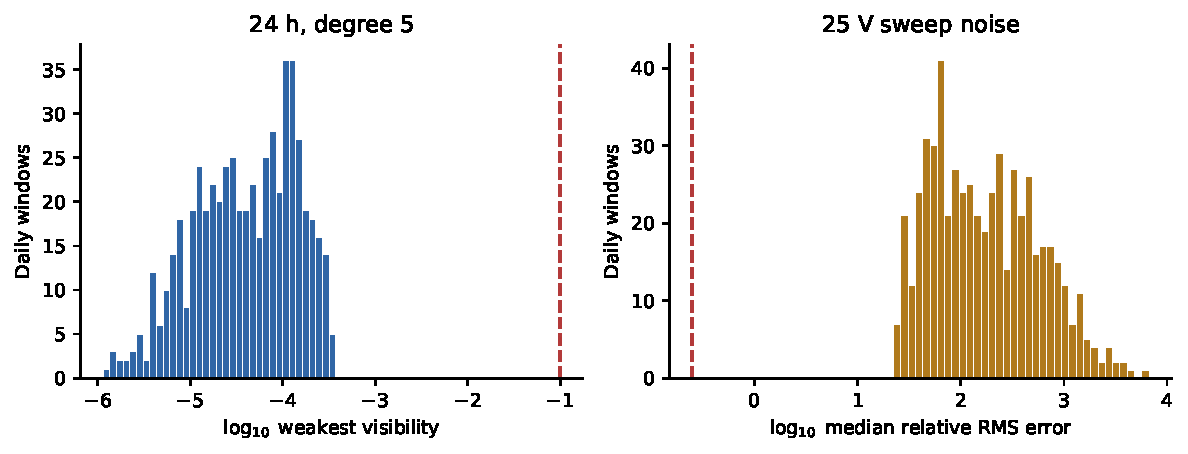
\includegraphics[width=0.82\textwidth]{../results/figures/primary-daily-failure.pdf}
\caption{Physical daily degree-5 visibility and recovery failure.}
\label{fig:primary}
\end{figure}

\subsection{Resolution boundary}

\begin{table}[ht]
\centering
\caption{Independent-window classes passing the frozen class gate.}
\label{tab:boundary}
\begin{tabular}{ll}
\toprule
Window duration & Passing maximum classes \\
\midrule
1 h & none \\
6 h & none \\
24 h & none \\
72 h & $L=1$ \\
168 h & $L=1,2,3$ \\
708.734112 h & $L=1,2,3,5,10$ \\
\bottomrule
\end{tabular}
\end{table}

The set of passing independent classes is exactly the same as in the original
run.  At 24 hours, degree 1 reaches only 80.7\% stable windows.  At 72 hours,
degree 2 passes recovery but not stability.  These cases illustrate why rank,
visibility, and recovery were required independently.

Whole-mission static fields pass through degree 20.  Their condition numbers
range from 1.37 to 3.75; the degree-20 median relative recovery error is
0.00938.  Shared constant-plus-synodic fields pass through degree 10.  The
degree-10 operator has rank $363/363$, condition number 3.13, weakest
visibility 0.729, and median recovery error 0.00832.  Removing the temporal
monopoles leaves rank $360/360$ and nearly identical diagnostics.

\begin{figure}[ht]
\centering
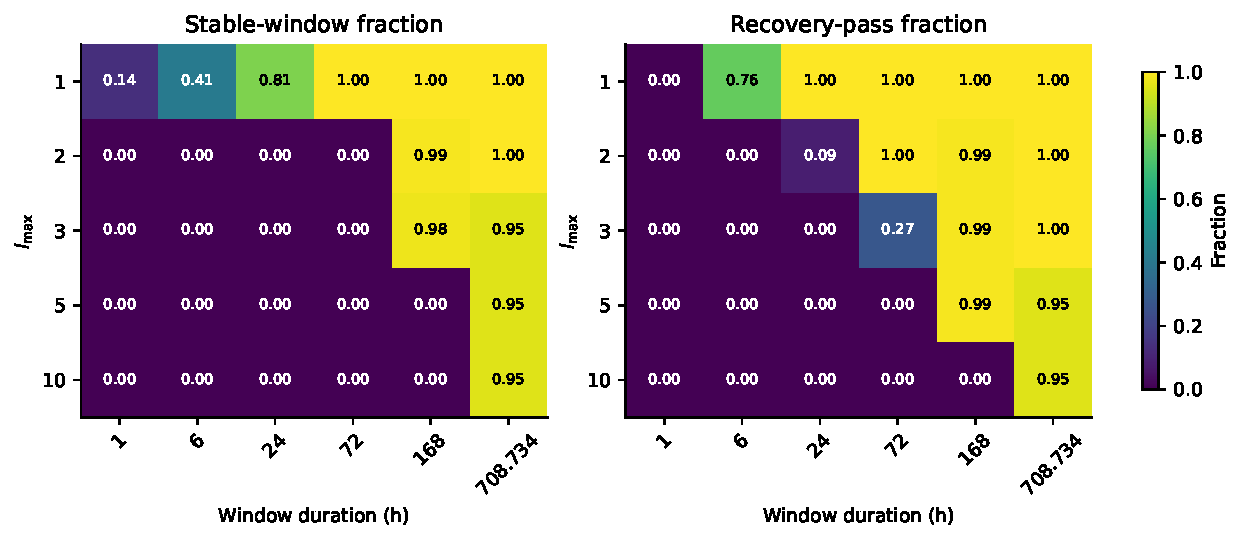
\includegraphics[width=0.82\textwidth]{../results/figures/window-degree-boundary.pdf}
\caption{Recoverability boundary versus window duration and spatial degree.}
\label{fig:boundary}
\end{figure}

\subsection{Sensitivity, blocked validation, and localized fields}

Every daily geometry sensitivity has 0\% stable and 0\% recovery-passing
windows.  This includes corrected and old equatorial native cohorts, their
exact paired cohort, legacy attitude, frame-mixed submitted geometry, midpoint
reduction, complete sweeps, solar co-rotation, contrast-only fields, and both
row-duplication assumptions.  Solar co-rotation raises median visibility to
$1.442\times10^{-4}$ but remains nearly 700 times below the 0.1 gate.

All 34 shared-model blocked fits are full rank.  Static degree-5 global median
errors span 0.263--0.315~V and shared synodic errors span 0.480--0.533~V.  Daily
degree-5 blocked fits tell the opposite story: contiguous-time holdouts have
29.1~kV median global error but 22.1~V held-out sampled error; longitude
holdouts have 17.7~kV global error but 9.7~V sampled error.  Local predictive
agreement is therefore insufficient evidence for a constrained global map.

Degree-5 representations of 15--30 degree localized caps have irreducible
approximation bias of 80.1 and 41.1~V, respectively, at 100~V truth RMS.
Median global reconstruction errors range from 100~V to 15.7~kV and
90th-percentile errors reach 161~kV, even when sampled residuals are small.

\section{Comparison with the original run}

\begin{table}[ht]
\centering
\caption{Key original and corrected diagnostics.}
\label{tab:comparison}
\begin{tabular}{lrr}
\toprule
Diagnostic & Original & Corrected \\
\midrule
Connected canonical sweeps & 399,643 & 389,317 \\
Median daily weakest visibility & $4.519\times10^{-5}$ & $4.449\times10^{-5}$ \\
Static degree-20 condition & 3.881 & 3.753 \\
Synodic degree-10 condition & 3.205 & 3.131 \\
Daily stable / recovery windows & 0 / 0 & 0 / 0 \\
Frozen decision & C & C \\
\bottomrule
\end{tabular}
\end{table}

The coordinate correction is not numerically negligible: it changes
footprints by tens to hundreds of kilometers and removes 2.58\% of the old
connected cohort.  Nevertheless, the median daily visibility changes by only
$-1.56$\%, the passing class boundary is identical, and corrected
mission-integrated controls are marginally better conditioned.  Outcome C is
therefore robust to the discovered coordinate defect.

Numerical cross-checks support this interpretation.  The primary and duplicate
grid paths agree exactly in stability and recovery fractions, with median
visibility difference $1.25\times10^{-17}$.  The constant block of the temporal
cache agrees with the spatial basis to $2.67\times10^{-15}$, and direct sampled
temporal evaluation agrees exactly.  Area-weighted grid evaluation gives
99.99746~V for representative nominal 100~V witness fields.

\section{Gauge, limitations, and interpretation}

The electron measurement is spacecraft-relative.  If unknown spacecraft
potential $u(t)$ is added to the model, its offset columns duplicate the
spatial $\ell=0$ column and matching temporal monopole columns.  The absolute
potential problem is exactly rank deficient in those directions.  Passing
contrast-only classes establish geometric identifiability of spatial
variation under their temporal assumptions, not absolute lunar potential.

The 25~V noise scale, Gaussian independence, and oracle sweep scalar are audit
assumptions, not measurement validation.  Experiment 008 does not establish
that loss-cone fitting produces unbiased sweep potentials or calibrated
uncertainties.  It also cannot exclude temporal model discrepancy: real
variability outside a static or single-synodic model can alias into its fitted
coefficients.

The scientifically defensible statement is consequently narrower than ``no
global information'' but stronger than a warning about regularization:
independent daily degree-5 global fields are not recoverable from LP ER
sampling, while substantially longer windows and compact shared temporal
models are conditionally identifiable.  Those passing operators should be
carried forward only after measurement-level experiments establish defensible
sweep values, uncertainties, and model-discrepancy treatment.

\section{Reproducibility record}

The replay uses run identifier \texttt{eclipj2000-v1}.  Large caches live in an
isolated artifact namespace; compact results, figures, freezes, and this
supplement live under the tracked replay directory.  The principal cache
hashes are:
\begin{quote}
\scriptsize\ttfamily
geometry: cb47bc11c3bae8fd89eacf1d946db06310f18692c0ff2b5863fcb4dc14eefa62\\
spatial: 19100c26e64890e9020044bee46ab7e572a6d31af53dcd9c3b606b83c066953e\\
temporal: e5f7a7345db7e4f53565e5d1037c20e52eaf96f18f32b811c3ccae3b32cf3fdb
\end{quote}
The original experiment outputs remain unchanged and independently hashable.

\end{document}
